\documentclass[tikz,border=5pt]{standalone}
\usepackage[T1]{fontenc}
\usepackage{lmodern,amsmath,amssymb}
\usetikzlibrary{arrows.meta,calc,positioning,fit,backgrounds,shapes.geometric,matrix,decorations.pathreplacing,patterns}
\definecolor{ink}{gray}{0.08}
\definecolor{wash}{gray}{0.965}
\definecolor{soft}{gray}{0.45}
\tikzset{box/.style={draw=ink,line width=.65pt,fill=white,align=center,inner sep=4pt,outer sep=0pt,font=\small},flow/.style={draw=ink,line width=.65pt,-{Latex[length=1.8mm,width=1.3mm]},rounded corners=2pt},annotation/.style={font=\scriptsize,text=soft,align=center},groupbox/.style={draw=soft,dashed,line width=.45pt,fill=wash}}
\begin{document}
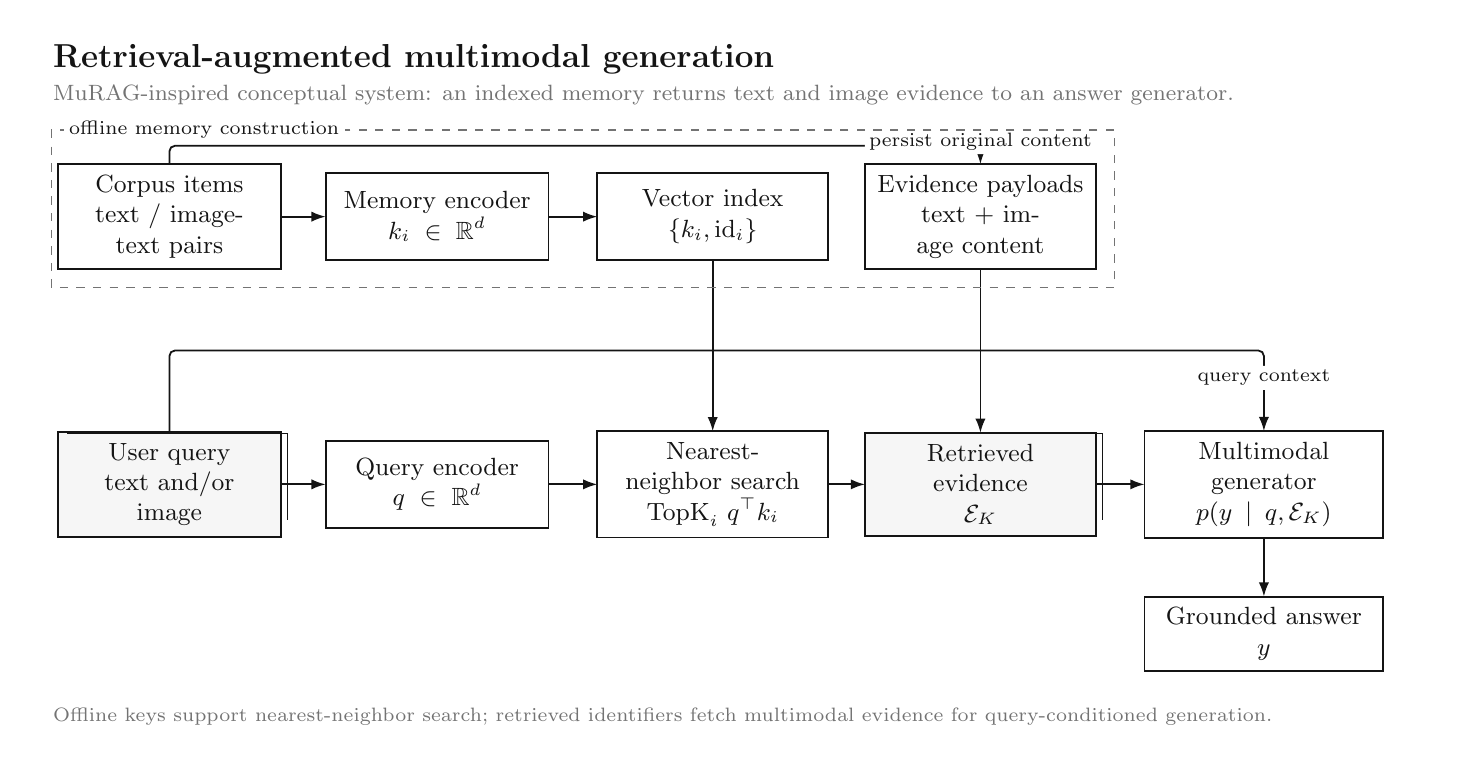
\begin{tikzpicture}[x=1cm,y=-1cm,font=\rmfamily,text=ink]

\path[use as bounding box] (0,0) rectangle (18,9);
\node[anchor=west,font=\large\bfseries] at (.2,.4) {Retrieval-augmented multimodal generation};
\node[anchor=west,font=\footnotesize,text=soft] at (.2,.85) {MuRAG-inspired conceptual system: an indexed memory returns text and image evidence to an answer generator.};
\begin{pgfonlayer}{background}
\end{pgfonlayer}
\node[box,minimum width=2.8cm,minimum height=1.1cm,text width=2.55cm] (corpus) at (1.8,2.4) {Corpus items\\text / image-text pairs};
\node[box,minimum width=2.8cm,minimum height=1.1cm,text width=2.55cm] (keys) at (5.2,2.4) {Memory encoder\\$k_i\in\mathbb{R}^{d}$};
\node[box,minimum width=2.9cm,minimum height=1.1cm,text width=2.65cm] (index) at (8.7,2.4) {Vector index\\$\{k_i,\mathrm{id}_i\}$};
\node[box,minimum width=2.9cm,minimum height=1.1cm,text width=2.65cm] (payload) at (12.1,2.4) {Evidence payloads\\text + image content};
\node[box,fill=wash,minimum width=2.8cm,minimum height=1.1cm,text width=2.55cm] (query) at (1.8,5.8) {User query\\text and/or image};
\draw[ink,line width=.4pt] (0.5000000000000001,5.15) -- (3.3000000000000003,5.15) -- (3.3000000000000003,6.25);
\node[box,minimum width=2.8cm,minimum height=1.1cm,text width=2.55cm] (qenc) at (5.2,5.8) {Query encoder\\$q\in\mathbb{R}^{d}$};
\node[box,minimum width=2.9cm,minimum height=1.2cm,text width=2.65cm] (search) at (8.7,5.8) {Nearest-neighbor search\\$\mathrm{TopK}_i\ q^{\top}k_i$};
\node[box,fill=wash,minimum width=2.9cm,minimum height=1.1cm,text width=2.65cm] (evidence) at (12.1,5.8) {Retrieved evidence\\$\mathcal E_K$};
\draw[ink,line width=.4pt] (10.75,5.15) -- (13.649999999999999,5.15) -- (13.649999999999999,6.25);
\node[box,minimum width=3.0cm,minimum height=1.2cm,text width=2.75cm] (gen) at (15.7,5.8) {Multimodal generator\\$p(y\mid q,\mathcal E_K)$};
\node[box,minimum width=3.0cm,minimum height=0.8cm,text width=2.75cm] (answer) at (15.7,7.7) {Grounded answer\\$y$};
\begin{pgfonlayer}{background}
\draw[flow] (corpus.east) -- (keys.west);
\draw[flow] (keys.east) -- (index.west);
\draw[flow] (corpus.north) -- (1.8,1.5) -- (12.1,1.5) -- (payload.north) node[midway,above,fill=white,inner sep=1.5pt,font=\scriptsize] {persist original content};
\draw[flow] (query.east) -- (qenc.west);
\draw[flow] (qenc.east) -- (search.west);
\draw[flow] (index.south) -- (search.north);
\draw[flow] (search.east) -- (evidence.west);
\draw[flow] (payload.south) -- (evidence.north);
\draw[flow] (evidence.east) -- (gen.west);
\draw[flow] (gen.south) -- (answer.north);
\draw[flow] (query.north) -- (1.8,4.1) -- (15.7,4.1) -- (gen.north) node[midway,above,fill=white,inner sep=1.5pt,font=\scriptsize] {query context};
\end{pgfonlayer}
\draw[draw=soft,dashed,line width=.45pt] (0.3,1.3) rectangle (13.8,3.3);
\node[anchor=west,font=\scriptsize,fill=white,inner sep=2pt] at (0.44999999999999996,1.3) {offline memory construction};
\node[anchor=west,align=left,font=\scriptsize,text=soft,text width=17.6cm] at (.2,8.75) {Offline keys support nearest-neighbor search; retrieved identifiers fetch multimodal evidence for query-conditioned generation.};
\end{tikzpicture}
\end{document}
